%!TEX root = ../thesis.tex

\section{提案手法の概要}

\begin{figure}[h]
  \centering
  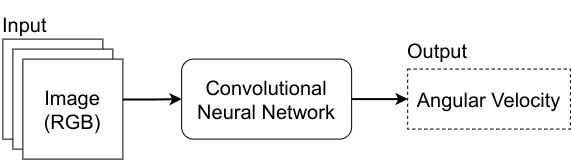
\includegraphics[keepaspectratio, scale=0.60] {images/RobotGuidance_simple_system.png}
  \captionsetup{justification=raggedright} % キャプションを左寄せに
  \caption{The trained network is used to generate the robot's yaw angular velocity from the RGB images}
  \label{Fig:RobotGuidance_simple_system}
\end{figure}

\begin{figure}[h]
  \centering
  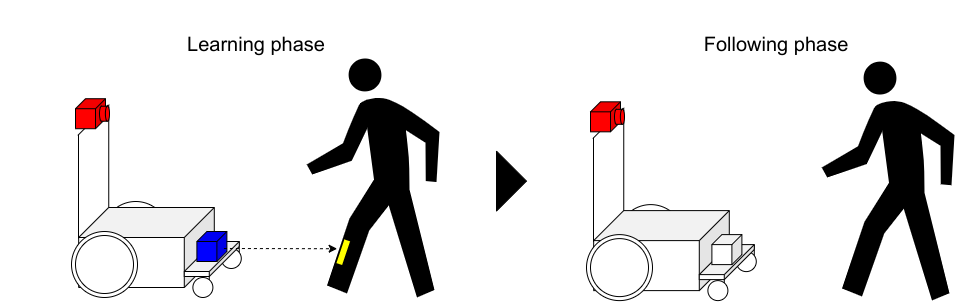
\includegraphics[keepaspectratio, scale=0.35] {images/RobotGuidance_all_system.png}
  \captionsetup{justification=raggedright} % キャプションを左寄せに
  \caption{Sequence of proposed method}
  \label{Fig:RobotGuidance_all_system}
\end{figure}

\begin{figure}[h]
  \centering
  \begin{minipage}[c]{65mm} 
      \centering
      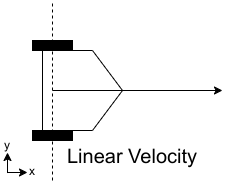
\includegraphics[height=40mm]{images/RobotGuidance_linear_velocity.png}
      \subcaption{Forward is fixed}
  \end{minipage}
  \begin{minipage}[c]{65mm} 
      \centering
      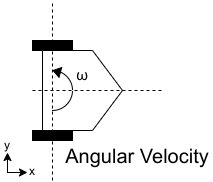
\includegraphics[height=40mm]{images/RobotGuidance_angular_velocity.png}
      \subcaption{Angular velocity changes depending on input}
  \end{minipage}
  \caption{Output robot actions}
  \label{Fig:RobotGuidance_velocity}
\end{figure}

\newpage
